\documentclass{sig-alternate} 
\usepackage{mathptmx} % This is Times font
\newcommand{\ignore}[1]{}
\usepackage{fancyhdr}
\usepackage[normalem]{ulem}
\usepackage[hyphens]{url}
\setlength{\emergencystretch}{10pt}
\usepackage{graphicx}
\usepackage{multirow}
\usepackage{breakurl}
\usepackage{tabularx}
\usepackage{balance}
\usepackage[nocompress]{cite}
\usepackage{subfig}
\usepackage{hyphenat}
\usepackage{xcolor}
\usepackage{soul}
\usepackage{dcolumn}
\newcolumntype{d}{D{.}{.}{2.1}}
\usepackage{pifont}
%\usepackage{flushend}
\usepackage{booktabs}
\usepackage{tikz}
\usepackage{siunitx}
\newcommand*\mycirc[1]{{\large \ding{\numexpr201+#1\relax}}}
% Always include hyperref last
% \usepackage[bookmarks=true,breaklinks=true,letterpaper=true,colorlinks,linkcolor=black,citecolor=blue,urlcolor=black]{hyperref}
% required to break long URLS sanely
% \PassOptionsToPackage{hyphens}{url} \usepackage{hyperref}
\expandafter\def\expandafter\UrlBreaks\expandafter{\UrlBreaks% save the current one 
\do\a\do\b\do\c\do\d\do\e\do\f\do\g\do\h\do\i\do\j% 
\do\k\do\l\do\m\do\n\do\o\do\p\do\q\do\r\do\s\do\t% 
\do\u\do\v\do\w\do\x\do\y\do\z\do\A\do\B\do\C\do\D% 
\do\E\do\F\do\G\do\H\do\I\do\J\do\K\do\L\do\M\do\N% 
\do\O\do\P\do\Q\do\R\do\S\do\T\do\U\do\V\do\W\do\X% 
\do\Y\do\Z\do\*\do\-\do\~\do\'\do\"\do\-}%

% Ensure letter paper
\pdfpagewidth=8.5in
\pdfpageheight=11in
\pagenumbering{arabic}

%%%%%%%%%%%---SETME-----%%%%%%%%%%%%%
\newcommand{\microsubmissionnumber}{265}
%%%%%%%%%%%%%%%%%%%%%%%%%%%%%%%%%%%%

\newcommand*\circled[1]{\tikz[baseline=(char.base)]{
  \node[shape=circle,draw,inner sep=1pt] (char) {#1};}}

\title{NUMA-Aware GPUs\\Towards Plug-and-Play Performance Scalability}

\author{
Ugljesa Milic$^{\mp\ddagger}$,
Oreste Villa$^{\dagger}$,
Evgeny Bolotin$^{\dagger}$,
Akhil Arunkumar$^{\dagger\star}$,\\\\
Eiman Ebrahimi$^{\dagger}$,
Aamer Jaleel$^{\dagger}$,
Alex Ramirez$^{\dagger\ast}$,
David Nellans$^{\dagger}$
\\\\
$^{\mp}$Universitat Polit\`ecnica de Catalinya (UPC), $^{\ddagger}$Barcelona Supercomputing Center (BSC), \\
$^{\dagger}$NVIDIA, $^{\star}$Arizona State University, and $^{\ast}$Google\\
}

\begin{document}

\maketitle
\pagestyle{plain}

\textbf{Summary.} With Moore's law limiting the transister growth of 
next-generation GPU accelerators, system architects must
embrace multi-socket designs in order to significantly increase the core count and memory 
bandwidth of future GPUs. However, maintaining the expected uniform memory 
system performance (of a single-GPU) in multi-GPU systems without significant 
application re-factoring is a major impediment to the adoption of multi-socket GPU
systems. As a result, we believe that within the next 10 
years GPU vendors will be forced to adopt programmer transparent runtimes that 
aggregate multiple physically discrete GPUs to form a single large virtual 
GPU, while also attempting to minimize the NUMA effects inherent in these designs.

In this work we investigate the impact that NUMA effects will have on 
transparent multi-GPU systems and show that several changes are needed to 
both the GPU interconnect and cache architectures to achieve good performance 
scalability. We show that application phase effects can be exploited, allowing 
individual GPU sockets to dynamically optimize their individual interconnect and cache 
policies, minimizing the impact of NUMA effects. Our programmer transparent NUMA-aware 
GPU\footnote{\textbf{Original version appears in MICRO 2017:} \\ Ugljesa Milic, 
Oreste Villa, Evgeny Bolotin, Akhil Arunkumar, Eiman Ebrahimi, Aamer Jaleel, 
Alex Ramirez, David Nellans. "Beyond the Socket: NUMA-Aware GPUs", in 
proceedings of 2017 IEEE/ACM International Symposium on Microarchitecture (MICRO 
2017)} outperforms a single GPU by 1.5$\times$, 2.3$\times$, and 3.2$\times$ 
while achieving 89\%, 84\%, and 76\% of theoretical application scalability in 
2, 4, and 8 sockets designs respectively. Transparent multi-GPU systems are 
implementable using today's GPUs, and when combined with our proposed 
NUMA-aware architectural designs will provide the easiest path to 
dramatically increased GPU throughput.

\textbf{Motivation and Prior Work.} Over the past 10 years, GPUs have become a 
significant component in datacenter, high performance computing (HPC), and 
machine learning installations; improving the performance of these workloads by 
exploiting their abundant data parallelism. Nevertheless, with GPUs nearing
reticle limitations for maximum die size and transistor density growth rate 
slowing down, developers looking to scale the performance of their single GPU 
programs are in a precarious position. Today, multi-GPU programming models do 
support explicit programming of two or more GPUs, but it is challenging to 
manage multiple GPUs and requires significant modification to single 
GPU optimized codebases.  At the same time, GPUs are expanding beyond the traditional 
PCIe peripheral interface to enable more efficient interconnection protocols 
between both GPUs and CPUs and GPUs and GPUs. Future high bandwidth GPU-to-GPU interconnects, 
possibly using improved communication protocols, will lead to system designs 
with closely coupled groups of GPUs that can efficiently share memory at fine 
granularity.

\begin{figure}[t]
	\centering
	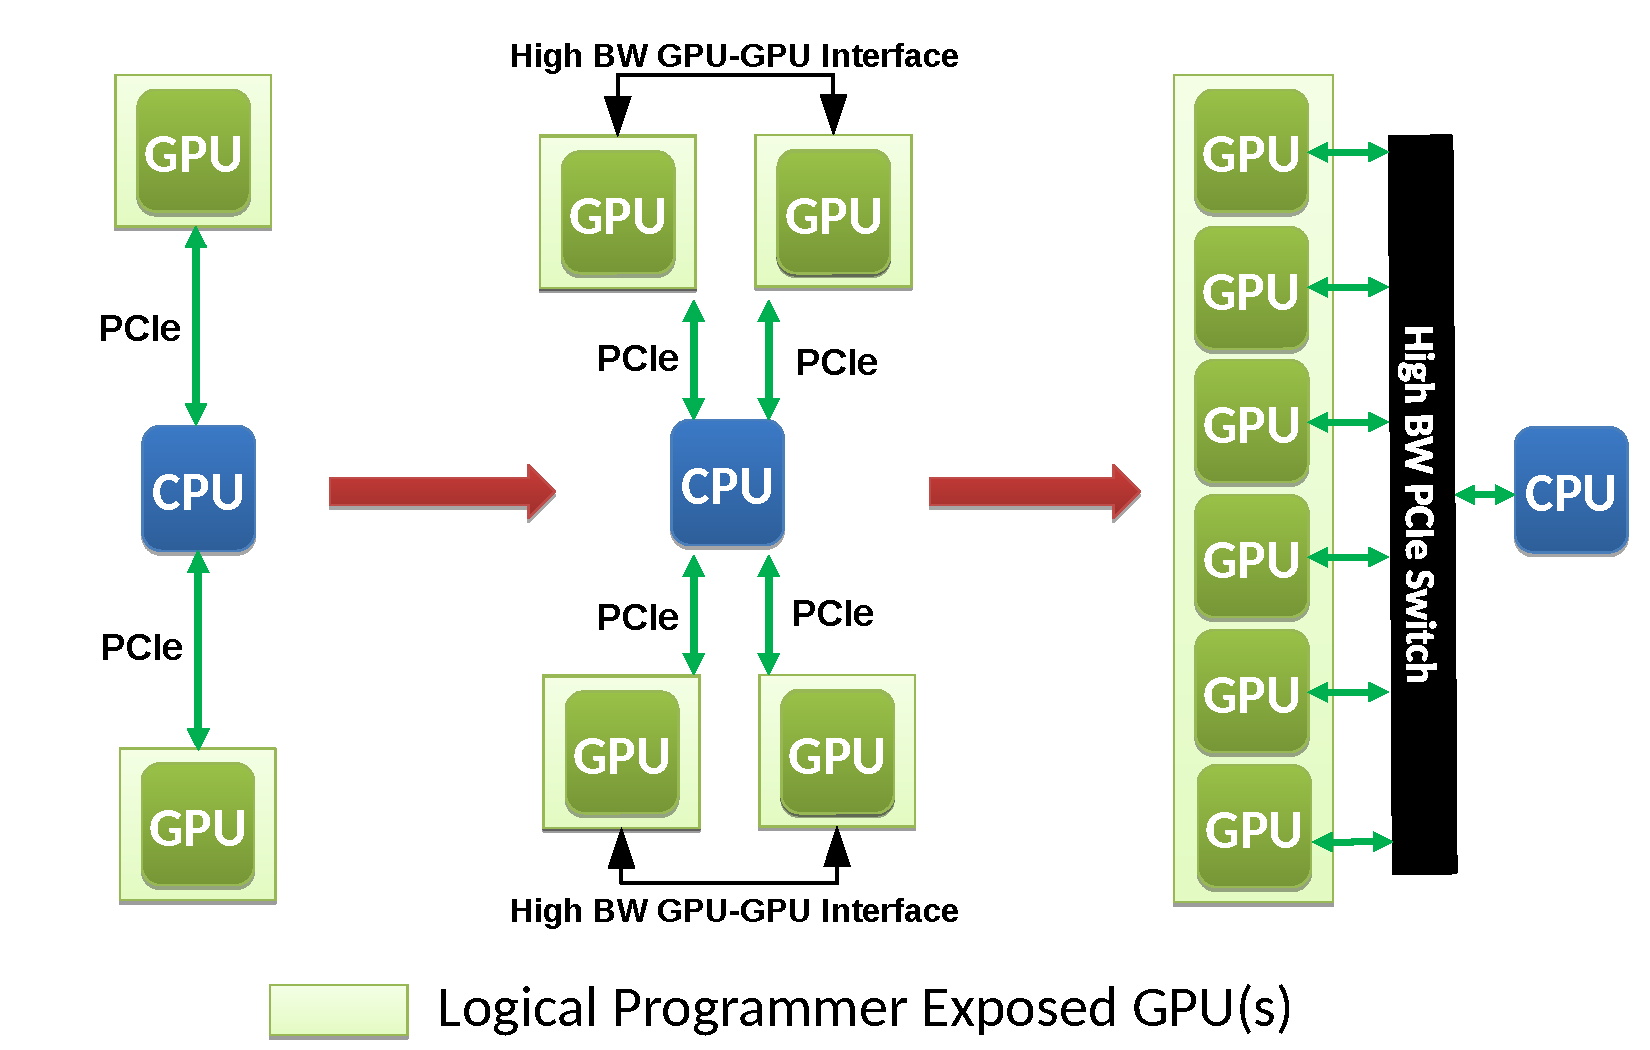
\includegraphics[width=1.0\columnwidth]{figures/inter_gpu_connections.pdf}
	\caption{The evolution of GPUs from traditional discrete PCIe devices to 
		single logical, multi-socket accelerators.}
	\vspace{-0.25in}
	\label{fig:systemdiagram}
\end{figure}

The onset of these multi-socket GPU systems will provide a pivot point for GPU 
and system vendors. On one hand, vendors can continue to expose GPUs as 
individual resources and force developers to use multiple programming paradigms 
to leverage these GPUs. On the other, vendors can expose multi-socket designs as 
a single programmer transparent NUMA-GPU resource as shown in 
Figure~\ref{fig:systemdiagram}.  By extending the single GPU programming model 
to multi-socket GPUs, applications can scale beyond the constraints of Moore's 
law, while simultaneously retaining the programming interface which GPU 
developers have become accustomed.  Extracting significant performance 
scalability while maintaining existing programming interfaces is a desireable 
combination and will see widespread adoption by end-users.

\begin{figure*}[!t]
	\centering
	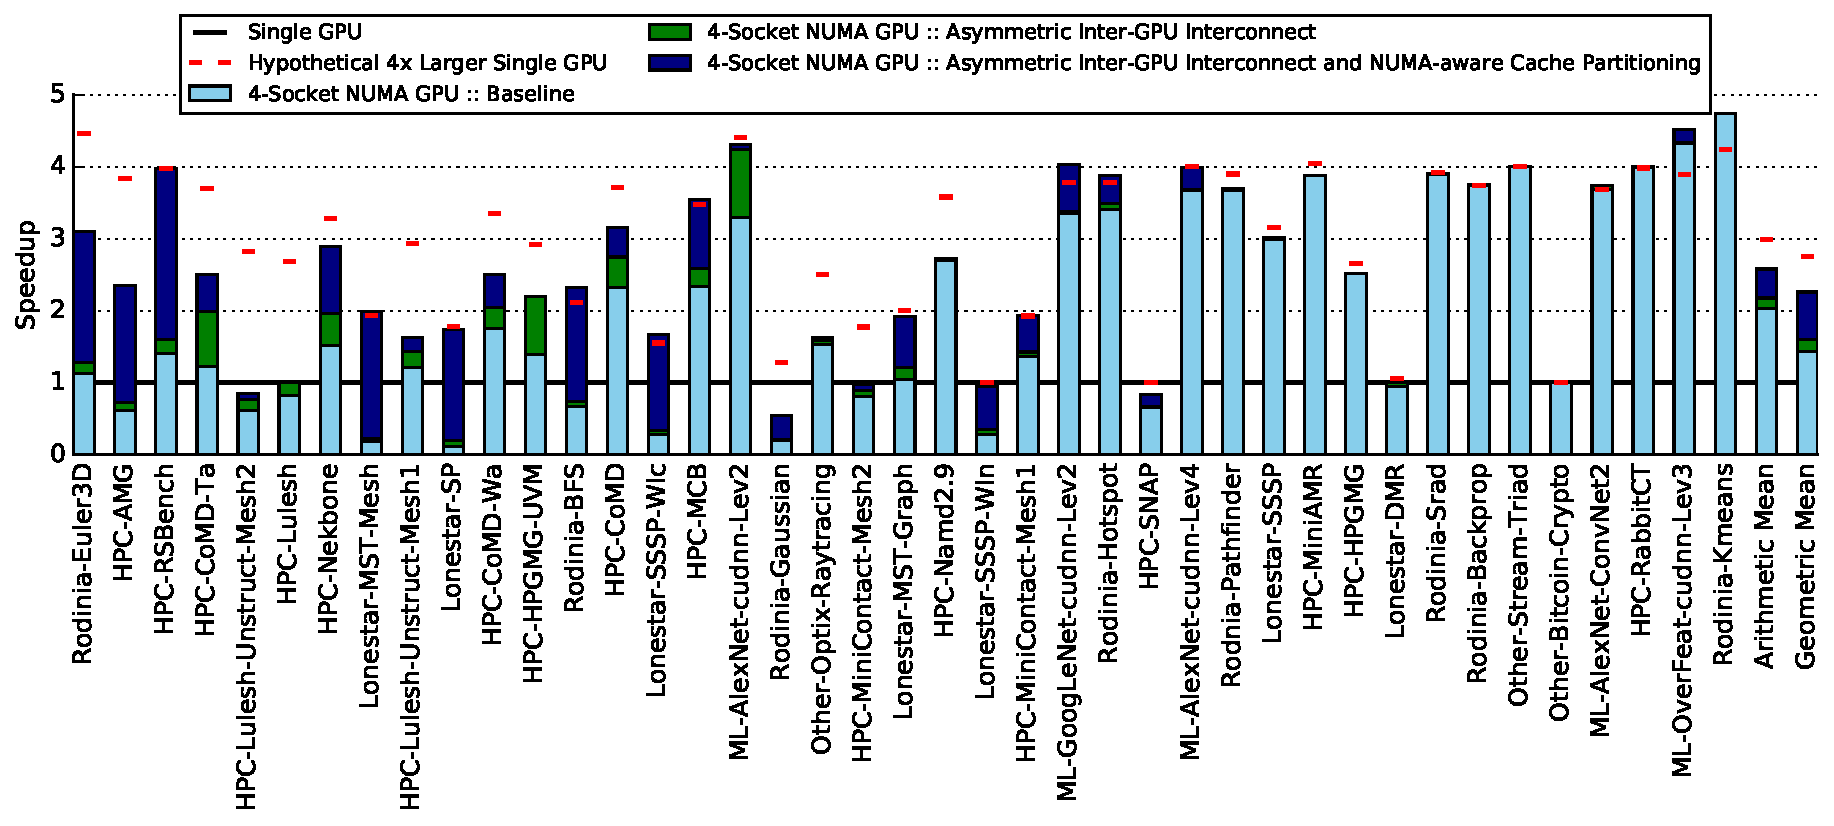
\includegraphics[width=1.0\textwidth]{figures/plot_final_speedup_WB_nvlink_first.pdf}
	\caption{Final NUMA-aware GPU performance compared to a single GPU and 4$\times$ 
	larger single GPU with scaled resources.}
	\vspace{-0.225in}
	\label{fig:combined}
\end{figure*}

Researchers have previously examined aggregating multiple GPUs together under a single 
programming model~\cite{lee2013transparent,Cabezas2015}; however this work was 
done in an era where GPUs had limited memory addressability and relied on high 
latency, low bandwidth CPU-based PCIe interconnects. As a result, prior work 
was able to improve the multi-GPU programming experience but was unable to achieve
performance scalability. Building upon this work, we show that in a new
era of unified CPU and GPU memory~\cite{UVM}, cache line addressable high 
bandwidth interconnects~\cite{NVLINK}, and dedicated GPU and CPU socket PCB 
designs, scalable transparent multi-GPU performance is now achievable if GPU
architectures become NUMA-aware.

\vspace{-.05in}
\section{NUMA-aware GPU Designs}

Our work shows that NUMA bandwidth (not latency) between GPUs is the primary
performance limitation in a transparent multi-GPU system and we provide two orthoginal
architectural optimizations to overcome this challenge.

\textbf{Dynamically Reconfigurable Interconnects:} In NUMA-GPU systems, we 
observe that applications have different utilization of egress and ingress 
channels on both a per GPU-socket basis and during different execution phases. 
To increase NUMA-bandwidth, we propose to dynamically rebalance multi-lane link assignments on a
per-GPU basis. We suggest replacing unidirectional lanes with bi-directional 
lanes that can be turned around on demand. During kernel 
execution the link load balancer then periodically samples the BW saturation of each 
link. If the lanes in one direction are underutilized, while the lanes in the 
opposite direction are saturated, the load balancer reconfigures and 
reverses the direction of one of the unsaturated lanes after quiescing all 
packets on that lane. This sample and reconfigure process stops only when 
directional utilization is not oversubscribed or all but one lane is configured 
in a single direction.

\textbf{NUMA-Aware Cache Partitioning:} To improve performance in situations 
where dynamic link rebalancing is ineffective (both directions saturated), 
decreasing the amount of traffic that crosses the low bandwidth NUMA channels is 
the only other option. GPUs today typically utilize memory-side L2 caches as an effective 
bandwidth filter to DRAM, but for NUMA-GPUs this is a bad architectural design point. 
Because memory-side caches only cache accesses that originate in their local 
memory, they cannot cache data from other NUMA zones and save precious NUMA 
interconnect traffic. Thus to minimize inter-GPU bandwidth we propose repurposing 
this L2 cache capacity and instead using a new
NUMA-aware cache partitioning algorithm that balances the allocation of cache capacity
in the GPU to remote or local memory based on the bandwidth saturation of local
and remote memories.  We show that simple schemes such as static cache partitioning
or fully contended caches underperform NUMA-aware caches that are aware of the NUMA
bandwidth differences in the system.

\textbf{Performance Results: }Figure~\ref{fig:combined} shows the overall 
improvement transparent multi-GPUs can achieve when designed for NUMA-awareness. 
Our baseline is a 4-socket SW locality-optimized GPU with contiguous 
thread block scheduling and first touch page migration~\cite{Arunkumar2017}. We 
observe that on the right side of the graph, some workloads can achieve or 
surpass the case of a hypothetical 4$\times$ larger monolithic GPU. However, the 
applications on the left side show a large gap between the baseline multi-GPU design 
and theoretical performance that NUMA-aware GPU architectures can achieve.  
We observe that our proposed optimizations are largely complimentary and help maximize 
performance across a wide range of workloads. When 
combined, our NUMA-aware multi-socket GPU achieves 2.1$\times$ improvement over a 
single GPU and 80\% improvement over a 4 socket multi-GPU without NUMA-awareness.

NUMA-Aware transparent multi-GPU technology may be most interesting because 
\textit{it allows users to scale performance by simply plugging in additional 
GPUs.} We show that on average a dual-socket NUMA GPU achieves 1.5$\times$ 
speedup, while 4 sockets and 8 sockets achieve 2.3$\times$ and 3.2$\times$ 
speedups respectively over a single GPU. Comparing our NUMA-aware GPU 
implementation to the scaling that applications would achieve on a hypothetical 
(but unbuildable) large single GPU, NUMA-aware multi-GPUs can achieve 89\%, 
84\%, and 76\% the efficiency in 2, 4, and 8 
socket configurations respectively. This high efficiency factor indicates that 
our design is able to largely eliminate the NUMA penalty in future multi-socket 
GPU designs, though further improvements are possible.

\vspace{-.05in}
\section{Long Term Impact} Over the last decade single GPU performance has 
scaled thanks to a significant growth in per-GPU transistor count and DRAM 
bandwidth. Unfortunately, transistor density is slowing significantly and 
integrated circuit manufacturers are not providing roadmaps beyond \SI{7}{nm}.
Porting applications to multi-GPU programming models is difficult and presents
a significant barrier to adoption for many GPU-compute users.  This work provides
the blueprint for an easily achievable way to enable unmodified workload performance
scaling from one to as many as eight GPUs.
Today, multi-GPU compute nodes are already available, e.g.\@ NVIDIA's DGX-1 
system with 8 GPUs and the US Department of Energy Summit and Sierra HPC 
nodes with 6 GPUs. However, only a small subset of applications benefit from an increased number of GPUs 
within a compute
node. Our NUMA-aware transparent multi-GPU design allows the code of \textit{all} GPU accelerated 
workloads to immediately strong-scale on multiple GPUs.\@

For decades, the promise of parallel code has been performance scalability. 
This has been realized on single GPUs, but today that promise does not hold on 
well on multiple GPUs, because crossing the socket boundary with efficient memory referencing 
was not well handled. By combining dynamic page placement into memory at 
runtime~\cite{UVM} and interconnects with cache line granularity~\cite{NVLINK}, 
our proposal enables transparent access to remote memory without the need to 
modify application source code, extending the promise of parallel programming across
the socket boundary.  While other techniques are being proposed to improve the transistor
count of single GPUs, such as multi-chip-modules GPUs~\cite{Arunkumar2017}, those
approaches do not have the same level of scalability as a transparent multi-GPU
system which can scale to 4,8, or 16 times larger than today's biggest GPUs (if
the NUMA overheads can be overcome or hidden through microarchitectural improvements).
At the limit, future GPU-centric compute nodes are likely to be comprised of multiple-sockets
of multi-chip-module GPUs that have been made NUMA-aware at the architectural level, achieving
the best of both on-package and off-package scalability.  Performance
improvements that are 2-8 times beyond current GPUs will not be achieved through traditional
architectural improvements, full system system architectures such as multi-GPU systems, is 
where significant gains will be sourced.

We believe this work will be impactful both within the field of computer architecture, but 
more importantly, outside the field of computer architecture.  Within our 
specialty, transparent multi-socket GPU execution will enable a wave of research 
similar to the 25 year (and on going) trend of multi-socket CPU 
research. While similar concepts are likely to be re-applied within the GPU domain, 
the NUMA bottleneck for GPUs is not a discrepancy between local and remote 
memory access latency but instead bandwidth;  instead of exploiting instruction 
level parallelism to hide the memory wall, it must now be done using energy-efficient 
data and thread level parallelism, while considering locality as a first class principle. 
There are many challenging problems and 
open questions (thread block scheduling, dynamic page migration and replication, 
prefetching policies, making other parts of GPU architecture NUMA-aware, etc.\@) 
that need to be studied by a research community willing to address them.

Outside our field,  GPUs are the preeminant compute acceleration technique used in
machine learning, computer vision, and autonomous robotics.  The algorithms
used in these fields iterate at such a rapid pace, that deep learning frameworks (for example)
have little time to heavily optimize for a single piece, or even generation, of GPU hardware;
before new techniques are invented.  This means that many machine learning frameworks
are not yet multi-GPU capable, despite the best efforts of GPU vendors. NUMA-aware
transparent multi-GPUs can provide a immediate shot in the arm to ML researchers
across the globe by providing a 2-8$\times$ improvement in both GPU memory capacity and
throughput, while requiring no modification to these rapidly iterating code-bases.
We believe no technique proposed in the architecture community today has the same potential
for performance upside, with such little overhead to the programmer, and is realizable on
such a short timeline. \textbf{Citation:} \textit{In 2017 Milic et al. provided a blueprint for NUMA-Aware
multi-socket GPUs and demonstrated that thanks to their inherently parallel design both at
the language and architectural level, unmodified GPU applications can see 2-8$\times$ improvements 
in performance simply by increasing the number of GPUs within the system.}

\bibliographystyle{IEEEtran}
\vspace{-0.1in}
\bibliography{main}
\end{document}
